\documentclass{standalone}
\usepackage{tikz}
\usetikzlibrary{snakes, decorations.pathmorphing}
\tikzset{snake it/.style={decorate, decoration=snake}}
\tikzset{snake soft/.style={decorate, decoration=snake, segment length=10cm}}

\begin{document}
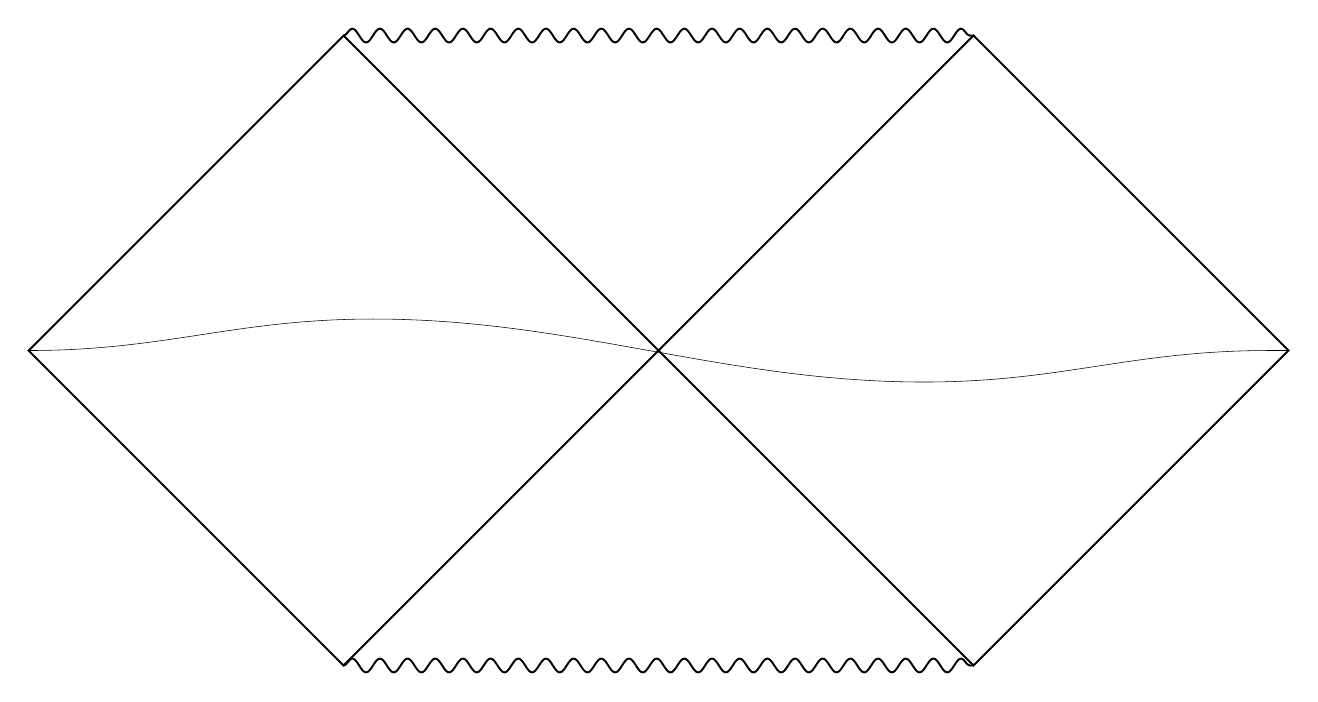
\begin{tikzpicture}
\node (I)    at ( 4,0)   {};
\node (II)   at (-4,0)   {};
\node (III)  at (0, 2.5) {};
\node (IV)   at (0,-2.5) {};

\path  % Four corners of left diamond
  (II) +(90:4)  coordinate      (IItop)
       +(-90:4) coordinate      (IIbot)
       +(0:4)   coordinate      (IIright)
       +(180:4) coordinate      (IIleft)
       ;

\path % Four conners of the right diamond (no labels this time)
   (I) +(90:4)  coordinate (Itop)
       +(-90:4) coordinate (Ibot)
       +(180:4) coordinate (Ileft)
       +(0:4)   coordinate (Iright)
       ;
% No text this time in the next diagram
\draw[line width=0.7pt]  (Ileft) -- (Itop) -- (Iright) -- (Ibot) -- (Ileft) -- cycle;
\draw[line width=0.7pt]  (IIleft) -- (IItop) -- (IIright) -- (IIbot) -- (IIleft) -- cycle;

% Squiggly lines
\draw[line width=0.7pt,snake it] (IItop) -- (Itop);
\draw[line width=0.7pt,snake it] (IIbot) -- (Ibot);

% Foliation line
\draw[line width = 0.2pt, snake=snake, segment amplitude=4mm, segment length=14cm] (IIleft) -- (Iright); 


\end{tikzpicture}
\end{document}